\documentclass[journal]{IEEEtran}
%\usepackage[retainorgcmds]{IEEEtrantools}
%\usepackage{bibentry} 
\usepackage{tablefootnote}
\usepackage{xcolor,soul,framed} %,caption
\colorlet{shadecolor}{yellow}
% \usepackage{color,soul}
\usepackage[pdftex]{graphicx}
\graphicspath{{../pdf/}{../jpeg/}}
\DeclareGraphicsExtensions{.pdf,.jpeg,.png}
\usepackage[cmex10]{amsmath}
%Mathabx do not work on ScribTex => Removed
%\usepackage{mathabx}
\usepackage{array}
\usepackage{mdwmath}
\usepackage{mdwtab}
\usepackage{eqparbox}
\usepackage{url}
\usepackage{nomencl}
\makenomenclature
\usepackage{multirow}
\usepackage{cite}

%\bstctlcite{IEEE:BSTcontrol}
\makeatletter
\newcommand*{\rom}[1]{\expandafter\@slowromancap\romannumeral #1@}
\makeatother

\usepackage{etoolbox}
\renewcommand\nomgroup[1]{%
  \item[\bfseries
  \ifstrequal{#1}{A}{\textit{A. General}}{%
  \ifstrequal{#1}{B}{\textit{B. Indexes}}{%
  \ifstrequal{#1}{C}{\textit{C. Parameters}}{%
  \ifstrequal{#1}{D}{\textit{D. Variables}}{%
  \ifstrequal{#1}{E}{\textit{E. Sets}}{%
  \ifstrequal{#1}{F}{\textit{F. Operators}}{}}}}}}%
]}

%=== TITLE & AUTHORS ====================================================================
\begin{document}
\bstctlcite{IEEEexample:BSTcontrol}
    \title{Imbalance Constrained Crossphase Quadratic OPF for Optimal Integration of EV Chargers and PV Inverters in Meshed and Radial Distribution Systems}
  \author{Araz~Bagherzadeh~Karimi,~\IEEEmembership{Student Member,~IEEE,}
      Reza~Deihimi~Kordkandi,~\IEEEmembership{Student Member,~IEEE,}\\
      Farrokh~Aminifar,~\IEEEmembership{Member,~IEEE,}
      Mohsen~Hamzeh,~\IEEEmembership{Member,~IEEE,}
      

  \thanks{}
  \thanks{}% <-this % stops a space
  \thanks{}%
  \thanks{}% <-this % stops a space
  \thanks{}}  


% The paper headers
\markboth{IEEE TRANSACTIONS ON POWER SYSTEMS, VOL.~XX, NO.~XX, DECEMBER~XXXX
}{Araz \MakeLowercase{\textit{et al.}}: Imbalance Constrained Crossphase ...}


% ====================================================================
\maketitle

% === ABSTRACT ====================================================================
% =================================================================================
\begin{abstract}

Inverter-Based distributed energy resources specially Photovoltaic devices (PVs) and electric vehicle charge stations (EVCS) in the sequel of the power-electronics interface, provide unprecedented flexibility to the system such as the ability to transfer line power across phases. This paper proposes a comprehensive framework for per phase optimal active, reactive, and cross-phase power flow dispatch of PVs and EVCSs. The optimization problem is targeted to maximize the firm benefit of DSO subject to the operational constraints including unbalanced situation tolerability of loads. The problem is formulated as a quadratic objective function with linearized constraints to maintain the tractability with a large number of per phase meshed buses and constraints. A new approximate equation of voltage unbalance factor (VUF) is introduced and used alongside existing linearized equations of other constraints. The applicability of the framework is validated via the unbalanced multi-phase IEEE 33 bus and IEEE 192 bus systems. The results show that the cross-phase capability of PVs and EVs and VUF consideration can significantly helps the system to satisfy the voltage imbalance limits while increasing the maximum profit in both their operational and nonoperational modes.

\end{abstract}


% === KEYWORDS ====================================================================
% =================================================================================
\begin{IEEEkeywords}
\h{Distributed Energy Resources, Electric Vehicle Charge Stations, Cross-phase power flow, Power Quality, Voltage Imbalance Factor}
\end{IEEEkeywords}


%=====Nomenclature Table==================================================================


\nomenclature[A]{\(OF\)}{Objective function}
\nomenclature[B]{\(\varphi,\gamma\)}{Index of phases}
\nomenclature[B]{\(\ell\)}{Index of lines}
\nomenclature[B]{\(s\)}{Index of a slack bus}
\nomenclature[B]{\(i\),\(j\)}{Index of buses}
\nomenclature[C]{\(\alpha_{i_{mn}}^{\varphi\gamma}\),\(\beta_{i_{mn}}^{\varphi\gamma}\),\(\delta_{i_{mn}}^{\varphi\gamma}\)}{VUF quadratic approximation coefficients}
\nomenclature[C]{\(P_{i_{ld}}^{\varphi},Q_{i_{ld}}^{\varphi}\)}{Active and reactive powers consumed by load}
\nomenclature[C]{\(P_{i_{PV}}^{sun}\)}{Maximum available active power of a PV}
\nomenclature[C]{\(S_{i}^{inv} _{PV}, S_{i}^{inv} _{EV}\)}{Phase to neutral rated powers of  a PV and EV}
\nomenclature[C]{\(P_{i_{EV}}^{sch}\)}{Scheduled consumed active power of an EVCS}
\nomenclature[C]{\(R_{ij}^{\varphi\gamma},X_{ij}^{\varphi\gamma}\)}{Total resistance and reactance of line from bus \textit{i} to bus \textit{j} and phase $\varphi$ to phase $\gamma$}
\nomenclature[C]{\(V_{i}^{min},V_{i}^{max}\)}{Minimum and maximum permissible voltage in bus \textit{i}}
\nomenclature[C]{\(S_{ij}^{max}\)}{Phase to neutral rated apparent power flow of line from bus \textit{i} to bus \textit{j}}
\nomenclature[C]{\(VUF_{i}^{max}\)}{Maximum permissible VUF in bus \textit{i}}
\nomenclature[C]{\(V_i\)}{Three-phase Voltage phasor vector}
\nomenclature[C]{\(c_1^s,c_2^s,c_3^s\)}{Cost coefficients of the power provided by the upper voltage system in slack bus \textit{s}}

\nomenclature[D]{\(V_i ^{\varphi},\theta_i^{\varphi}\)}{Voltage magnitude and angle in bus \textit{i} and phase $\varphi$}
\nomenclature[D]{\(P_{i}^{\varphi}_{inject},Q_{i}^{\varphi}_{inject}\)}{The injected active and reactive powers}
\nomenclature[D]{\(P_{i_{PV}}^{\varphi},Q_{i_{PV}}^{\varphi}\)}{Active and reactive powers injected from PV}
\nomenclature[D]{\(P_{i_{EV}}^{\varphi},Q_{i_{EV}}^{\varphi}\)}{Active and reactive powers injected from EV}
\nomenclature[D]{\(P_{ij}^{\varphi\gamma},Q_{ij}^{\varphi\gamma},S_{ij}^{\varphi\gamma}\)}{Active, reactive and apparent power flows of line from bus \textit{i}, phase $\varphi$ to bus \textit{j} and phase $\varphi$ to phase $\gamma$} 
\nomenclature[D]{\(VUF_{i}\)}{Voltage imbalance factor in bus number \textit{i}}
\nomenclature[C]{\(w', w_i, w\)}{Weight factors of objective function}
\nomenclature[D]{\(VUF_{i}^{apr}\)}{Voltage imbalance factor approximation in bus number \textit{i}}
\nomenclature[E]{\(N\)}{Set of buses}
\nomenclature[E]{\(\phi\)}{Set of phases}
\nomenclature[E]{\(L\)}{Set of lines}
\nomenclature[E]{\(S\)}{Set of Slack Buses}
\nomenclature[F]{\(\{A\}^{+},\{A\}^{-}\)}{Positive and negative sequence of the three phase phasor vector A}
\nomenclature[F]{\(\hat A\)}{Linear approximation of A}
\printnomenclature[2.8cm]





% === I. INTRODUCTION =============================================================
% =================================================================================
\section{Introduction}

\IEEEPARstart{M}{inimizing} the loss and the operational cost of distribution networks is a critical goal for distribution system operators (DSOs). Distribution networks, by nature, are unbalanced in terms of voltages and currents because of having untransposed lines \cite{paranavithana2009global} in distribution feeders and integration of single-phase generators and loads with highly probabilistic behavior. While voltage imbalance mostly impacts the costumers’ power quality, the current imbalance is one of the main causes of loss increase in distribution networks. Mitigation of current and voltage imbalance sources is a serious technical requirement and has drawn the attention of researchers for many years. We review the approaches revolving around the voltage and current imbalance compensation in the following.

  Based on \cite{kong2017three} we can decompose the origins of the imbalance into twofold classes: structural and random. The method focusing on the structural aspect includes network reconfiguration \cite{borozan1997,  morton2000efficient, dall2014sparsity, ding2015feeder, fu2018toward} and phase balancing \cite{zhu1998phase, chen1999optimal, siti2007reconfiguration}. These techniques, however, do not have real-time flexibility and continuous controllability for compensating the random component of imbalance. Static transfer system (STS) based methods are proposed to compensate for this \cite{ding2018per}. This method may impose switching transients and is less flexible than power electronics devices with continuous controllability. Device-based compensation has been broadly investigated in the literature and proved outstanding capability in mitigating the current imbalance \cite{valderrama2001reactive, pires2004unbalanced, salmeron2004compensation, xu2007voltage}. These techniques were rarely implemented in the past but their integrations are abruptly on the rise due to the proliferation of Distributed Energy Resources (PVs) and Electrical Vehicle Charge Stations (EVCSs).
  
Local control strategies for leveraging distributed energy PVs for imbalance compensation have been discussed in \cite{singh2010grid, weckx2015load}. These approaches, as expected, are highly effective but they still lack utilization of full capability of flexible power electronics resources due to the control with incomplete local information status. In the wake of cyber-physical distribution networks enabled by the vast deployment of communication systems, the operational strategies running over the network model with complete system-wide information turn into a real practice \cite{dall2012optimization, robbins2015optimal, araujo2013three, su2014optimal, nguyen2018exact, sheshyekani2019participation}. These methods accommodate the controllability of PV resources and seek to minimize the operation cost in the presence of distribution network imbalance. Voltage imbalance is tackled as a subsidiary objective function in the optimization problem. 

All of the methods mentioned in last paragraph mainly revolve around three-phase or single-phase PVs but non of them implements the cross-phase capability for the three-phase inverters in their models. In addition, they are either proposing a non-convex model which compromises the computational performance, or if they propose a convex model, it is only valid in radial topology and due to the rectangular model requirement for those simplifications, the highly non-linear non-convex VUF equation is ignored. Therefore, in this paper a novel feasible three-phase optimal power flow that can also include the above motioned overlooked aspects is tailored which includes these main features:

\begin{itemize}
    \item  Introducing a Convex (QP) three-phase optimal power flow that models bus voltages in polar form with magnitudes and angles and uses linearized load flow equations and capacity constraints that minimizes an objective function including total cost and a polynomial data driven approximation of VUF which is computationally fast and scalable because of convexity and can also be implemented in heavily meshed three-phase distribution networks.
\end{itemize}
\begin{itemize}
    \item Participating the ever-growing three- and single-phase EV chargers alongside with three- and single-phase PVs in optimal power flow operation not only to avoid their possible harmful operation but also exploiting the full capacity of installed devices to reduce cost and improve system conditions. 
\end{itemize}
\begin{itemize}
    \item Introducing Cross-phase operation in three-phase inverter models that can exploit the unused three-phase inverter capacity in terms of active and reactive power in different operational and non-operational modes in order to improve system conditions and reduce the cost even more.
\end{itemize}

Various sub-methods and scenarios are created, tested, and compared in IEEE 33 bus radial and 192 bus heavily meshed test systems. The provided results fully compare the scenarios, sub-methods, Inverter devices, and the two topologies in terms of cost, loss and VUF. The results Also create a starting point to address these critical questions for DSOs; 1) How much should an inverter or load owner pay for making system unbalanced. and 2) How much should be paid for an inverter owner for enabling the cross-phase operation.  

The remainder of this paper is organized as follows. Section \rom{2} formulates the proposed optimization problem. The computation implementation is described in \rom {3}. Section \rom{4} shows the parameter tuning while the results and the corresponding discussion are presented in section \rom{5}. Finally, conclusive remarks are presented in Section \rom{6}.



% === II. Problem Formulation ========================
% =================================================================================
\section{Problem Formulation}

The optimization problem is cast based on an OPF model with a single objective function and multiple physical and operational constraints including the imbalance limits. The convex form of the OPF model is employed here and the new constraints are convexified to be in line with the whole model trait.

\subsection {Power Flow model}

Three-phase power balance equations consisting of PV injection, EV interaction, and load consumption are expressed as:

\begin{equation}\label{P_ij_phigamma}
\begin{split}
\forall i\in N,\varphi\in\phi, \hskip 80pt\\
P_{i_{inject}}^{\varphi}+P_{i_{PV}}^{\varphi}=P_{i_{ld}}^{\varphi}+P_{i_{EV}}^{\varphi}+
\displaystyle\sum_{j|(i,j)\in L}\displaystyle\sum_{\gamma|\gamma\in\phi}P_{ij}^{\phi\gamma}
\end{split}
\end{equation}


\begin{center}
\begin{equation}\label{Q_ij_phigamma}
\begin{split}
\forall i\in N,\varphi\in\phi, \hskip 80pt\\ Q_{i_{inject}}^{\varphi}+Q_{i_{PV}}^{\varphi}=Q_{i_{ld}}^{\varphi}+Q_{i_{EV}}^{\varphi}+
\displaystyle\sum_{j|(i,j)\in L}\displaystyle\sum_{\gamma|\gamma\in\phi}Q_{ij}^{\phi\gamma}
\end{split}
\end{equation}
\end{center}

It is implicitly assumed in the framework that if a bus does not have a connected device (MV transformer, PV or EVCS) the corresponding active and reactive power related to that device is forced to be zero. In addition, the self and mutual impedance of all phases are also accounted in the three-phase active and reactive power balance equations. In (\ref{P_ij_phigamma}) and (\ref{Q_ij_phigamma}) the $P_{ij}^{\varphi\gamma}$ and $Q_{ij}^{\varphi\gamma}$ can be written as:

\begin{equation}\label{4}
P_{ij}^{\varphi\gamma}=
\frac
{
\begin{split}
\forall (i,j) \in L, \varphi,\gamma \in \phi \hskip 50pt\\
R_{ij}^{\varphi\gamma}(V_{i}^{\varphi})^2 -R_{ij}^{\varphi\gamma}V_{i}^{\varphi}V_{j}^{\gamma} \cos(\theta_{i}^{\varphi}-\theta_{j}^{\gamma})\\+ X_{ij}^{\varphi\gamma}V_{i}^{\varphi}V_{j}^{\gamma}\sin(\theta_{i}^{\varphi}-\theta_{j}^{\gamma})
\end{split}}
{\left(R_{ij}^{\varphi\gamma}\right)^2 + \left(X_{ij}^{\varphi\gamma}\right)^2}
\end{equation}

\begin{equation}\label{5}
Q_{ij}^{\varphi\gamma}= \frac
{
\begin{split}
\forall (i,j) \in L, \varphi,\gamma \in \phi \hskip 50pt\\
X_{ij}^{\varphi\gamma}(V_{i}^{\varphi})^2 -R_{ij}^{\varphi\gamma}V_{i}^{\varphi}V_{j}^{\gamma} \sin(\theta_{i}^{\varphi}-\theta_{j}^{\gamma})\\ +X_{ij}^{\varphi\gamma}V_{i}^{\varphi}V_{j}^{\gamma}\cos(\theta_{i}^{\varphi}-\theta_{j}^{\gamma})
\end{split}
}
{\left(R_{ij}^{\varphi\gamma}\right)^2 + \left(X_{ij}^{\varphi\gamma}\right)^2}
\end{equation}

In order to have a convex optimization model and tackle the problem via one of the efficient convex solvers, the linearized forms of (1) and (2) for single-phase distribution network are taken from \cite{yuan2016novel} and extended to three-phase unbalanced network. Equations (\ref{replaced_P_ij_phigamma}) and (\ref{replaced_Q_ij_phigamma}) denote branch active and reactive power losses and are defined based on the linearized power flow expression captured in (\ref{branch_active_power})-(\ref{linearized_Qij2}). As justifiable assumptions in distribution networks, it is assumed that the voltage magnitudes are around 1 p.u. and the angle differences of successive nodes are close to zero.

\begin{equation}\label{branch_active_power} \hskip 1pc
P_{ij}^{\varphi\gamma} \approx \hat{P_{ij-1}^{\varphi\gamma}} + \hat{P_{ij-2}^{\varphi\gamma}} = \hat{P}_{ij}^{\varphi\gamma}
\end{equation}

\begin{equation}\label{branch_reactive_power}
\hskip 1pc
Q_{ij}^{\varphi\gamma} \approx \hat{Q_{ij-1}^{\varphi\gamma}} + \hat{Q_{ij-2}^{\varphi\gamma}} = \hat{Q}_{ij}^{\varphi\gamma}
\end{equation}

\begin{equation}\label{linearized_Pij1}
\hat{P _{ij-1} ^{\varphi\gamma} }=\frac {r_{ij}^{\varphi\gamma}x_{ij}^{\varphi\gamma}} {r_{ij}^{\varphi\gamma2}+ x_{ij}^{\varphi\gamma2}} . \frac {V _{i} ^{\varphi} - V _{j} ^{\varphi}} {x _{ij} ^{\varphi\gamma}} = k _{ij-1} ^{\varphi\gamma} . \frac {V _{i} ^{\varphi} - V _{j} ^{\varphi}} {x _{ij} ^{\varphi\gamma}}
\end{equation}

\begin{equation}\label{linearized_Pij2}
\hat{P _{ij-2} ^{\varphi\gamma}}=\frac {x_{ij}^{\varphi\gamma2}} {r_{ij}^{\varphi\gamma2}+ x_{ij}^{\varphi\gamma2}} . \frac {\theta _{i} ^{\varphi} - \theta _{j} ^{\varphi}} {x _{ij} ^{\varphi\gamma}} = k _{ij-2} ^{\varphi\gamma} . \frac {\theta _{i} ^{\varphi} - \theta _{j} ^{\varphi}} {x _{ij} ^{\varphi\gamma}}
\end{equation}

\begin{equation}\label{linearized_Qij1}
\hat{Q _{ij-1} ^{\varphi\gamma}}=\frac {-r_{ij}^{\varphi\gamma}x_{ij}^{\varphi\gamma}} {r_{ij}^{\varphi\gamma2}+ x_{ij}^{\varphi\gamma2}} . \frac {\theta _{i} ^{\varphi} - \theta _{j} ^{\varphi}} {x _{ij} ^{\varphi\gamma}} =- k _{ij-1} ^{\varphi\gamma} . \frac {\theta _{i} ^{\varphi} - \theta _{j} ^{\varphi}} {x _{ij} ^{\varphi\gamma}}
\end{equation}

\begin{equation}\label{linearized_Qij2}
\hat{Q _{ij-2} ^{\varphi\gamma}}=\frac {x_{ij}^{\varphi\gamma2}} {r_{ij}^{\varphi\gamma2}+ x_{ij}^{\varphi\gamma2}} . \frac {V _{i} ^{\varphi} - V _{j} ^{\varphi}} {x _{ij} ^{\varphi\gamma}} = k _{ij-2} ^{\varphi\gamma} . \frac {V _{i} ^{\varphi} - V _{j} ^{\varphi}} {x _{ij} ^{\varphi\gamma}}
\end{equation}

As a result, (\ref{P_ij_phigamma}) and (\ref{Q_ij_phigamma}) can be replaced with (\ref{replaced_P_ij_phigamma}) and (\ref{replaced_Q_ij_phigamma}):

\begin{center}
\begin{equation}\label{replaced_P_ij_phigamma}
\begin{split}
\textit{P}_{i_{inject}} ^{\varphi} + P _{i_{PV}} ^{\varphi} =  P _{i_{ld}} ^{\varphi} +  P _{i_{EV}} ^{\varphi} \\ +\displaystyle\sum_{\ell|(i,j)\in L}\displaystyle\sum_{\gamma|\gamma\in\phi}\hat{P_{ij}^{\varphi\gamma}}
\end{split}
\end{equation}
\end{center}

\begin{equation}\label{replaced_Q_ij_phigamma}
\begin{split}
Q_{i_{inject}} ^{\varphi} + Q _{i_{PV}} ^{\varphi} =  Q _{i_{ld}} ^{\varphi} +  Q _{i_{EV}} ^{\varphi} \\ +\displaystyle\sum_{\ell|(i,j)\in L}\displaystyle\sum_{\gamma|\gamma\in\phi}\hat{Q_{ij}^{\varphi\gamma}}
\end{split}
\end{equation}

\subsection {Capacity constraint}

Capacity of distribution lines should guarantee the secure operation of the system. So, it can be written as:

\begin{equation}\label{line_capacity_constraint}
\begin{split}
\forall (i,j) \in \ell, \forall \varphi,\varphi \in \phi \hskip 25pt \\ S _{ij}^{\varphi\varphi}= \sqrt{P _{ij}^{\varphi\varphi2}+Q _{ij}^{\varphi\varphi2}} \leq S _{ij}^{max}
\end{split}
\end{equation}

In perspective of optimization problem parameters and variables, the equation (\ref{line_capacity_constraint}) is nonlinear and nonconvex. Therefore, linear approximation using piecewise linearization method \cite{akbari2016linear} is applied to maintain the linear and convex form of the problem and can be shown as:

\begin{center}
\begin{equation}\label{linearized_line_capacity_constraint}
\begin{split}
\forall h, h\in N, h\leq H, \forall(i,j) \in \ell, \forall\varphi,\varphi \in \phi \hskip 20pt \\
\left(\sin\left(\frac{360^{\circ}h}{H}\right)-\sin\left(\frac{360^{\circ}}{H}(h-1)\right)\right) P_{ij} ^{\varphi \varphi}-\\
\left(\cos\left(\frac{360^{\circ}h}{H}\right)-\cos\left(\frac{360^{\circ}}{H}(h-1)\right)\right) Q_{ij} ^{\varphi \varphi} \\ \leq S_{ij}^{max} \times \sin\left(\frac{360^{\circ}}{H}\right)
\end{split}
\end{equation}
\end{center}

\subsection{Voltage constraints: magnitude, imbalance factor}

The hard margin constraint voltage magnitude constraint is implemented as:

\begin{equation}\label{Voltage_magnitude_constraint}
\forall i, \varphi, \hskip 0.3pc i \in N, \varphi \in \phi, \hskip 1pc V_{min} \leq V_{i}^{\varphi} \leq V_{max}
\end{equation}

In (\ref{Voltage_magnitude_constraint}) the $V_{min}$ and $V_{max}$ are the voltage magnitude limits determined by the standards. In order to maintain power quality standards in unbalanced system the VUF standard is taken into consideration \cite{smith2009ieee}. Equation (\ref{VUF_Constraint}) demonstrates the definition of VUF.

\begin{equation}\label{VUF_Constraint}
VUF_{i} = \frac {|V_{i}^{-}|} {|V_{i}^{+}|} \leq VUF_{max}
\end{equation}

It should be mentioned that the hard margin implementation of highly non-linear VUF constraint is impossible in the convex optimization platform. Therefore the two options could be hard margin linear VUF approximation and soft margin quadratic approximation in a weighted-sum multiple objective optimization model. It is later discussed in \ref{Reg} that the latter is a more accurate approach, and therefore it is used as a VUF constraint basis in the presented formulation. The quadratic approximation of VUF can be shown as:

\begin{equation}\label{VUF_apr}
\begin{split}
VUF_{i} \approx VUF_{i}^{apr} 
\end{split}
\end{equation}
where:
\begin{equation}\label{VUF_apr_simplified}
\begin{split}
VUF_{i}^{apr} = \displaystyle\sum_{0\leq n\leq2}\displaystyle\sum_{0\leq m\leq<n}\displaystyle\sum_{\varphi,\gamma\in\phi}(\alpha_{i_{mn}}^{\varphi\gamma}(V_i^\varphi)^m(V_i^\gamma)^{n-m}\\ + \beta_{i_{mn}}^{\varphi\gamma}(V_i^\varphi)^m(\theta_i^\gamma)^{n-m} + \delta_{i_{mn}}^{\varphi\gamma}(\theta_i^\varphi)^m(\theta_i^\gamma)^{n-m})
\end{split}
\end{equation}


\subsection{Objective function}

Without loss of generality, the minimum operational cost of the system is sought here as (\ref{objective_function}). 

\begin{equation}\label{objective_function}
\begin{split}
OF \in R, \hskip 100pt \\ \hskip 0.5pt OF=\displaystyle\sum_{s\in S} (c_1^s + c_2^s P_{inject_s^{\varphi}}+ c_3^s (P_{inject_s^{\varphi}})^2)
\end{split}
\end{equation}

The active power injection of PVs and reactive power support of EVCSs are assumed to be costless. The objective functions can be readily tailored for meshed and multiple input distribution networks connected to MV systems with different cost terms. The objective function can also imply either minimization of the cost or maximization of firm benefit in the highly PV penetrated, and reverse power flow enabled systems. It is quite straightforward to replace it with maximum social welfare, maximum firm benefit, etc., or even proceed with multiple objectives, for the purpose of this paper the multi objective objective function is presented as (\ref{objective_function_VUF}).

\begin{equation}\label{objective_function_VUF}
\begin{split}
0\leq w',w_i \leq1
 , \; OF \in R,  \hskip 100pt \\ \hskip 0.5pt OF=w'\displaystyle\sum_{s\in S} (c_1^s + c_2^s P_{inject_s^{\varphi}}+ c_3^s (P_{inject_s^{\varphi}})^2)
\\+\displaystyle\sum_{i\in N} w_iVUF_{i}^{apr}
\end{split}
\end{equation}

  The weight coefficient $w_i$ is flexible to be customized for each bus to enable prioritizing the power quality constrain in certain buses. In other words, improve imbalance of a certain bus by only exploiting the existing system flexibility in the operation, without performing local modifications or installations. The weight coefficients used in the current approach is further discussed in \ref{Pareto}.  
  
   
\subsection {EVCS models}

EVCSs are considered both single- and three-phase in distribution systems. While they can flexibly provide reactive power based on system optimization, their consumed active power is assumed to be constant and adjusted based on the customer charging preference and the battery and inverter capability in a certain period of time. Nevertheless, they can provide some flexibility over consumed active power in each time interval thanks to their schedulability. Because we are targeted to perform the optimization in the near real time scope to handle random phenomena, we prefer to ignore this capability at least in the scope of this study.  The formulation of a single-phase EVCS in phase $ \kappa $ is shown in (\ref{single_phase_EVCSs_model1})-(\ref{single_phase_EVCSs_model3}). For simplification, EVCSs are shortened to EVs in the optimization formulations.

\begin{equation}\label{single_phase_EVCSs_model1}
\forall i, i \in N \hskip 1pc P_{i_{EV}}^{\kappa}=P_{i_{EV}}^{sch}
\end{equation}

\begin{equation}\label{single_phase_EVCSs_model2}
\forall i, i \in N \hskip 0.5pc \forall \varphi, \varphi \in \phi |\hskip 0.2pc \varphi \neq \kappa, \hskip 0.8pc P_{i}^{EV}= 0
\end{equation}

\begin{equation}\label{single_phase_EVCSs_model3}
\begin{split}
\forall i, i \in N \hskip 1pc -\sqrt{(S_{i_{EV}}^{inv})^2 - (P_{i_{EV}}^{\kappa})^2} \leq Q_{i_{EV}}^{\kappa}\\ \leq + \sqrt{(S_{i_{EV}}^{inv})^2 - (P_{i_{EV}}^{\kappa})^2}
\end{split}
\end{equation}

The variable $Q_{i_{EV}} ^{\kappa}$ can be derived based on the result of the optimization problem. Equations (\ref{three_phase_EVCSs_model1})-(\ref{three_phase_EVCSs_model3}) show the three-phase EVCS model and corresponding linearization. In the three-phase case, (\ref{single_phase_EVCSs_model1}) and (\ref{single_phase_EVCSs_model2}) are changed to (\ref{three_phase_EVCSs_model1}) in which the cross-phase active power transfer is also enabled.

\begin{equation}\label{three_phase_EVCSs_model1}
\forall i \in N, \hskip 2pt \displaystyle\sum _{\varphi \in \phi} P_{i_{EV}}^{\varphi} = P_{i_{EV}}^{sch}
\end{equation}

\begin{equation}\label{three_phase_EVCSs_model2}
\forall i, i \in N, \forall \varphi, \varphi \in \phi, \hskip 0.7pc \sqrt{(P_{i_{EV}}^{\varphi})^2 +(Q_{i_{EV}}^{\varphi})^2} \leq S_{i_{EV}}^{inv}
\end{equation}

\begin{equation}\label{three_phase_EVCSs_model3}
\begin{split}
\forall h, h \in H, \hskip 1pt \forall i, i \in N, \hskip 1pt \forall \varphi, \varphi \in \phi \hskip 30pt \\ \left(\sin\left(\frac{360^\circ h}{H}\right)- \sin\left(\frac{360^\circ}{H}(h-1)\right)\right)P_{i_{EV}}^{\varphi} \\
-\left(\cos\left(\frac{360^\circ h}{H}\right)- \cos\left(\frac{360^\circ}{H}(h-1)\right)\right)Q_{i_{EV}}^{\varphi} \\ \leq S_{i_{EV}}^{inv} \times \sin\left(\frac{360^\circ}{H}\right)
\end{split}
\end{equation}

Therefore, corresponding $P_{i_{EV}}^{\varphi}$(cross-phase active power) can be derived based on the optimization results as well as the $Q_{i_{EV}}^{\varphi}$. The noteworthy point is that even during the off hours of EVCSs, the active power can be transferred between phases like an active power line conditioner \cite{salmeron2004compensation}. This enables the EVCSs to provide more active ancillary services if needed and make them more economically reasonable.

\subsection{PVs model}

As same as the EVCSs, PVs are installed as three-phase and single-phase in distribution networks. While the three-phase PVs can contribute to the balancing and voltage magnitude control, the single-phase configurations may be harmful to the system power quality when used uncontrolled. Therefore, PV management not only can help the optimization problem to have enough flexibility to satisfy its objective, but also it is necessary for maintaining the power quality standards. The single-phase PV in phase $\kappa$ can be modeled as:

\begin{equation}\label{PV_model_1}
\forall i, i \in N, \hskip 2pt 0 \leq P_{i_{PV}}^{\kappa} \leq P_{i_{PV}}^{sun}
\end{equation}

\begin{equation}\label{PV_model_2}
\forall i, i \in N, \hskip 3pt \forall \varphi, \varphi \in \phi | \varphi \neq \kappa, \hskip 3pt P_{i_{PV}}^{\varphi}=0
\end{equation}

\begin{equation}\label{PV_model_3}
\forall i, i \in N, \hskip 5pt \sqrt{\left(P_{i_{PV}}^{\kappa}\right)^2 +\left(Q_{i_{PV}}^{\kappa}\right)^2} \leq S_{i_{PV}}^{inv}
\end{equation}

With the linear approximation, (\ref{PV_model_3}) can be replaced by:

\begin{equation}\label{linear_PV_model}
\begin{split}
\forall h, h \in H, \hskip 1pt \forall i, i \in N, \hskip 50pt \\ \left(\sin\left(\frac{360^\circ h}{H}\right)- \sin\left(\frac{360^\circ}{H}(h-1)\right)\right)P_{i_{PV}}^{\kappa} \\
-\left(\cos\left(\frac{360^\circ h}{H}\right)- \cos\left(\frac{360^\circ}{H}(h-1)\right)\right)Q_{i_{PV}}^{\kappa} \\ \leq S_{i_{PV}}^{inv} \times \sin\left(\frac{360^\circ}{H}\right)
\end{split}
\end{equation}

The corresponding $P_{i_{PV}}^{\kappa}$ and $P_{i_{PV}}^{\kappa}$ are derived as a result of the optimization problem. The three-phase PV model and the approximation are presented in (\ref{three-phase_PV_model_1}),(\ref{three_phase_PVs_model2}), and (\ref{three_phase_PVs_model3}), respectively:

\begin{equation}\label{three-phase_PV_model_1}
\forall i \in N, \hskip 3pt 
0 \leq \displaystyle\sum_{\varphi\in\phi} P_{i_{PV}}^{\varphi} \leq P_{i_{PV}}^{sun}
\end{equation}

\begin{equation}\label{three_phase_PVs_model2}
\forall i, i \in N, \forall \varphi, \varphi \in \phi, \hskip 0.7pc \sqrt{(P_{i_{PV}}^{\varphi})^2 +(Q_{i_{PV}}^{\varphi})^2} \leq S_{i_{PV}}^{inv}
\end{equation}

\begin{equation}\label{three_phase_PVs_model3}
\begin{split}
\forall h, h \in H, \hskip 1pt \forall i, i \in N, \hskip 1pt \forall \varphi, \varphi \in \phi \hskip 20pt\\ \left(\sin\left(\frac{360^\circ h}{H}\right)- \sin\left(\frac{360^\circ}{H}(h-1)\right)\right)P_{i_{PV}}^{\varphi} \\
-\left(\cos\left(\frac{360^\circ h}{H}\right)- \cos\left(\frac{360^\circ}{H}(h-1)\right)\right)Q_{i_{PV}}^{\varphi} \\ \leq S_{i_{PV}}^{inv} \times \sin\left(\frac{360^\circ}{H}\right)
\end{split}
\end{equation}

Finally, the $P_{i_{PV}}^{\varphi}$ and $Q_{i_{PV}}^{\varphi}$ can be derived as a result of the optimization problem. To sum up, the QP framework will be the minimization of the objective function of (\ref{objective_function}) subject to (\ref{replaced_P_ij_phigamma}), (\ref{replaced_Q_ij_phigamma}), (\ref{linearized_line_capacity_constraint}), (23)-(27), (29)-(31), (33), (34) and (36).

% ================= III. Computational Implementation===============================================


% ================= IV. Computational Implementation===============================================

\section{Computational Implementation}

\subsection {Input Structure and Test Cases}
The input Data structure is built and developed based on the MATPOWER structure \cite{zimmerman2010matpower}. The Matpower test case structure is modified from single line balanced to three phase unbalanced in order to be able to add the three-phase unbalanced test cases to the case library. For the purpose of this paper, two unbalanced standard systems are added to Matpower library; IEEE 33 Bus \cite{baran1989network} and the 192 LV buses of the IEEE 342-bus test system \cite{schneider2014ieee}. The two systems are chosen in such away that cover different voltage levels, bus numbers, topology type (meshed  or radial) and number of slack buses. Assuming the symmetrical configuration of its lines and cables, the IEEE 33-bus system is modified to be balanced three-phase system and then the loads are forced to be unbalanced by load intensity factor which will be defined later in the paper. However, the 192 LV buses of the IEEE 342-bus test system is inherently unbalanced and heavily meshed and connected to the MV system from different nodes in order to maintain reliability and satisfy the high load density. For the purpose of this research, single-phase and three phase PV and EVCs with different penetration levels are added to the test cases. Fig.~\ref{33_Bus_system} and ~\ref{192_Bus_system} demonstrate the  PV and EV locations of the mentioned systems respectively. It worth to mention that the location of EVs and PVs are occasionally overlapped to create a more intense test environment for the proposed method. The details of the test system parameters are elaborated in table \ref{table2}.

%%Figure%%33&192_Bus%%%%%%%%%%%%%%%%%%%%%%%%%%%%%%%%%%%%%%%%%%%%%%
\begin{figure}
\centering
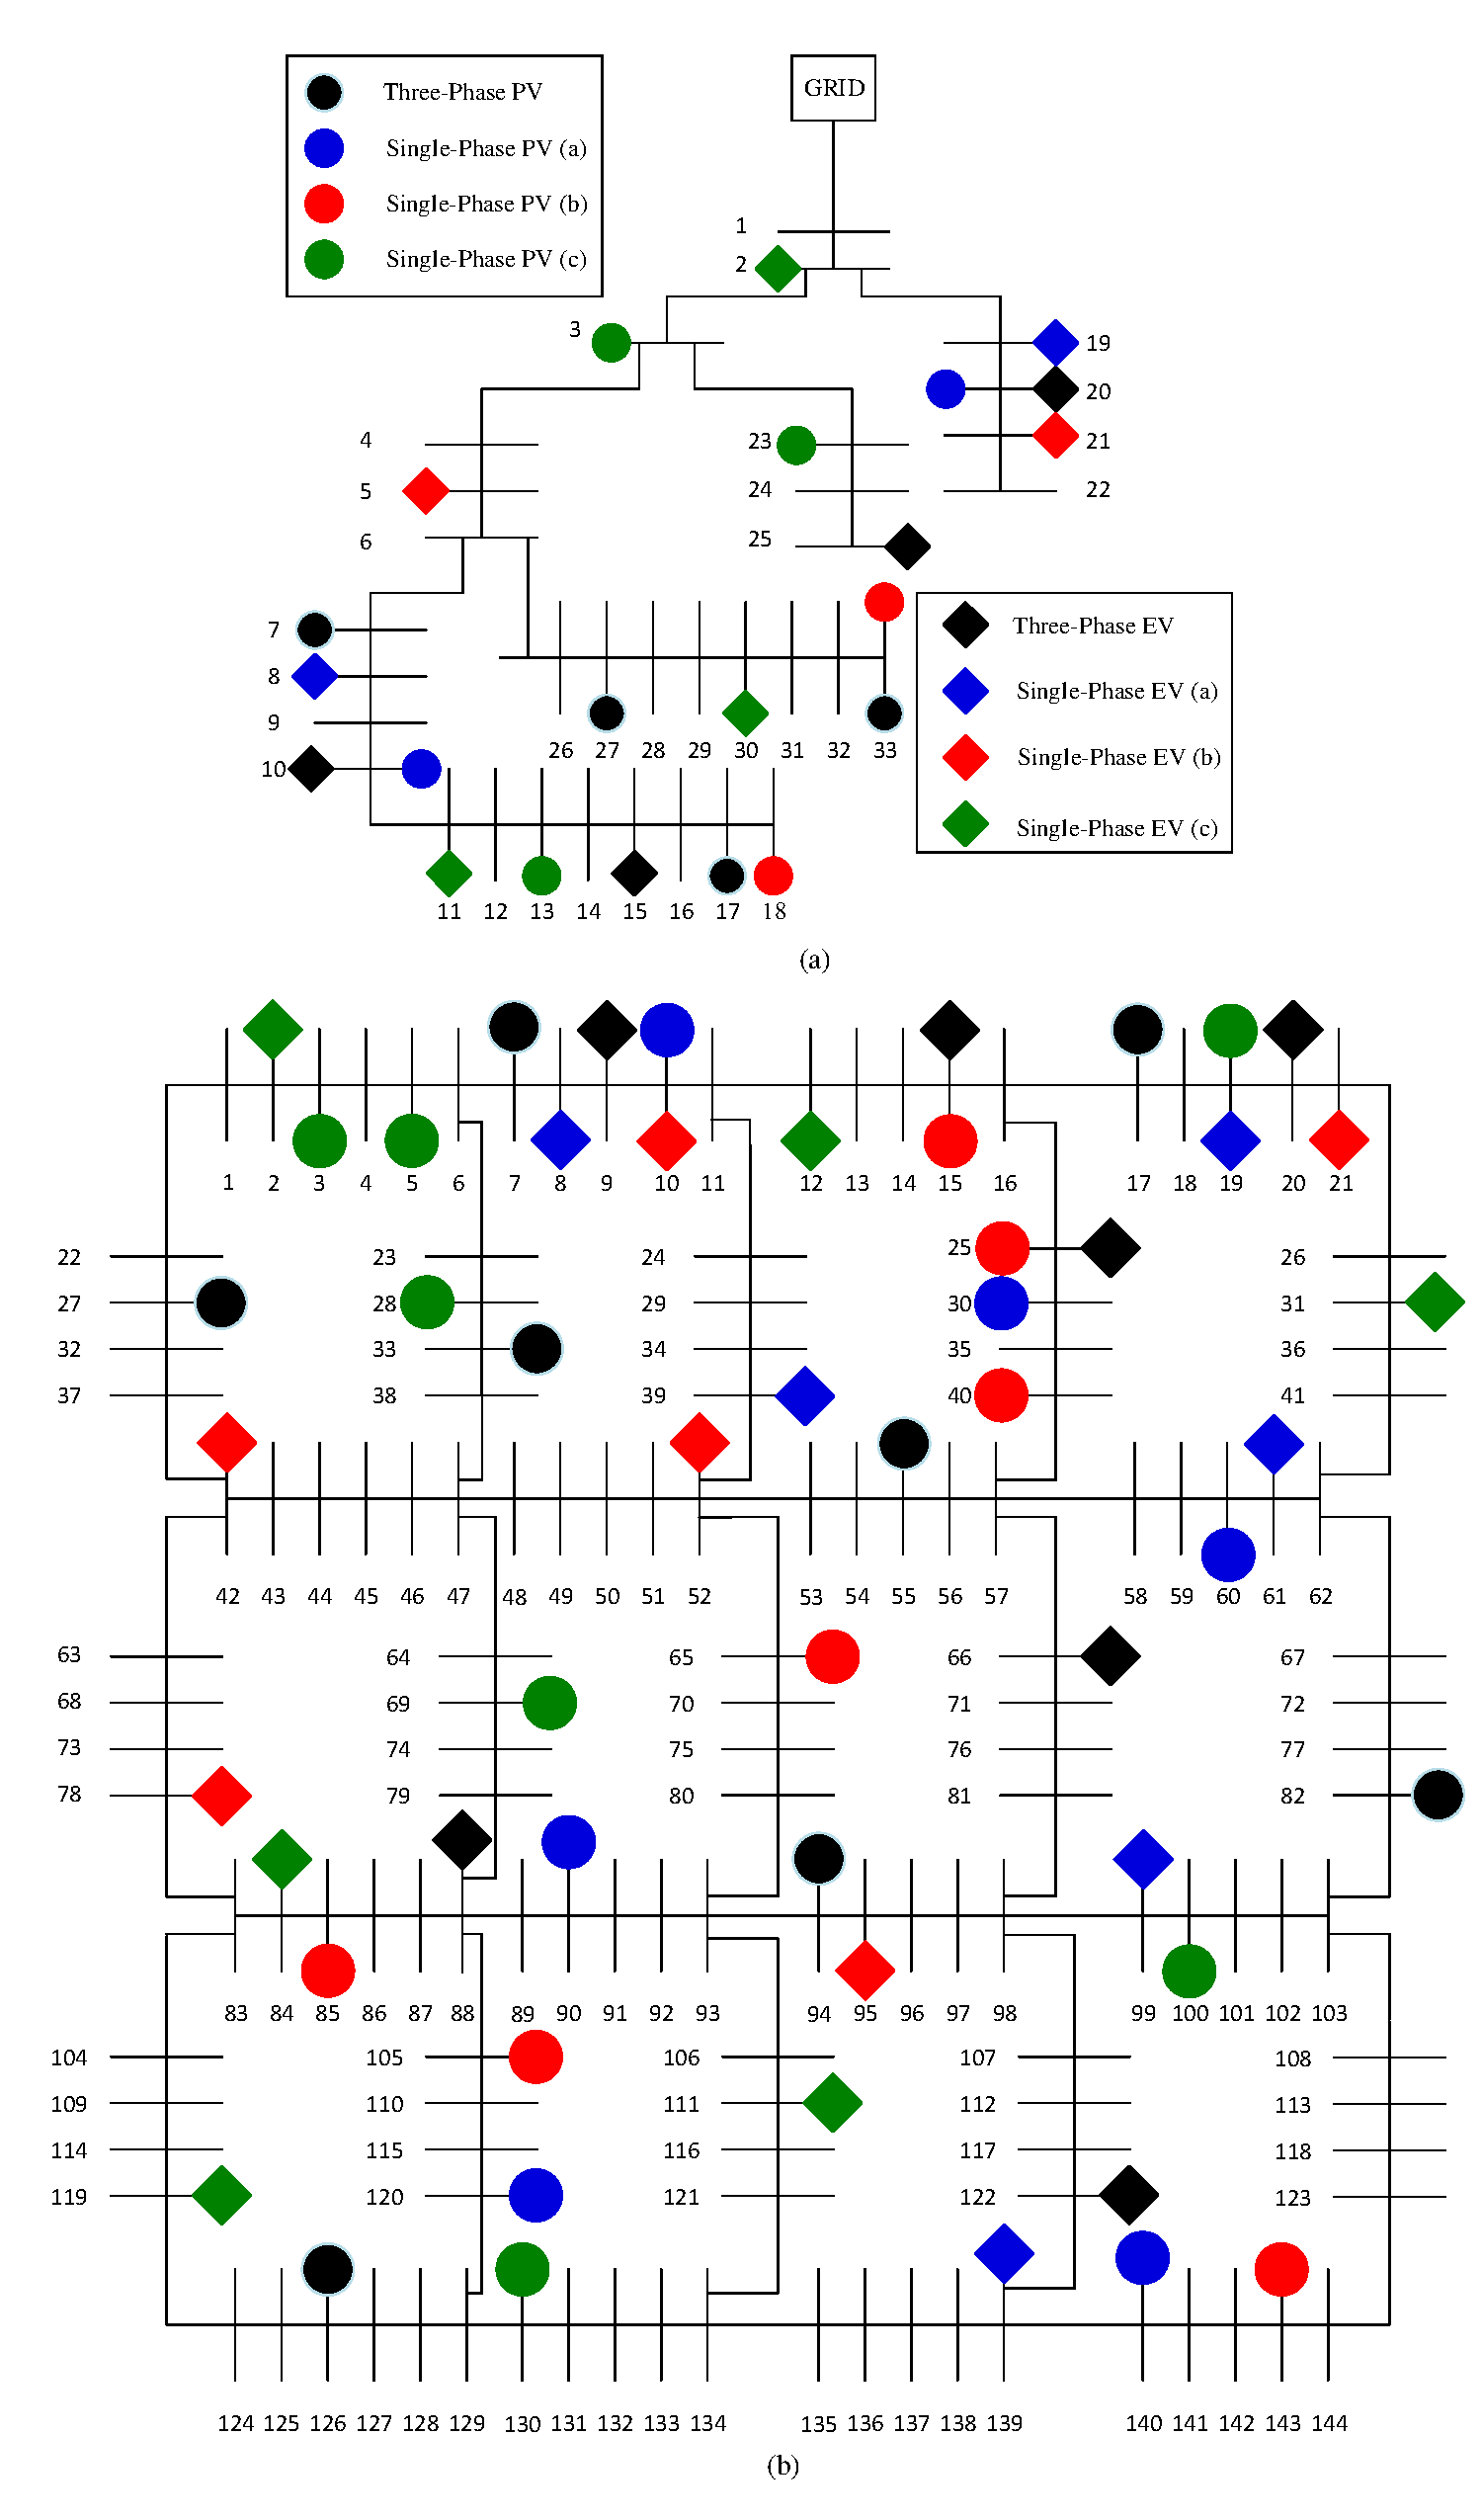
\includegraphics[width=9cm]{pdf/33 and 192 bus.pdf}
\caption{a) IEEE 33-bus, b) 192-bus system}
\label{33_Bus_system}
\end{figure}
%%%%%%%%%%%%%%%%%%%%%%%%%%%%%%%%%%%%%%%%%%%%%%%%%%%%%%%%%%%%%%
%%%%%%%%%%%%%%%%%%%%%%%%%%%%%%%%%%%%%%%%%%%%%%%%%%%%%%%%%%%%%%
%%%%%%%%%%%%%%%%%%%%Table2%%%%%%%%%%%%%%%%%5
\begin{table}
\begin{center}
\caption{System parameters}
\label{table2}
\begin{tabular}{ |p{3.5cm}|p{2cm}|p{2cm}| }
\hline
 \textbf{System} & \textbf{33-Bus} & \textbf{192-Bus} \\ 
 \hline\hline
 \textbf{L-n Voltage} & 12.6kv & 120 \\
 \hline
 \textbf{Min Voltage} & 0.9 p.u & 0.9 p.u\\
 \hline
 \textbf{Max Voltage} & 1.1 p.u & 1.1 p.u\\
 \hline
 \textbf{Cost Coefficient $c_{1}$} & 3 & 3 \\
 \hline
 \textbf{Cost Coefficient $c_{2}$} & 0.1 & 0.1 \\
 \hline
 \textbf{Cost Coefficient $c_{3}$} & 0 & 0 \\
 \hline
 \textbf{Base MVA} & 100MVA & 100MVA \\
 \hline
 \textbf{Sum of Loads} & 3.75MW & 2.9MW \\
 \hline
 \textbf{Average of Loads} & 0.11MW & 0.02MW \\
 \hline
 \textbf{Sum of Reactive Loads} & 2.3MW & 1.82MW \\
 \hline
 \textbf{Average of Reactive Loads} & 0.07MVAR & 0.012MVAR \\
 \hline
 
%\multirow{2}{8em}{\textbf{Three-phase EV Charger Capacity}}& \multirow{2}{*}{0.54MVA}& \multirow{2}{*}{0.54MVA} \\ &   &  \\

{\textbf{Three-phase EV Capacity}}& 0.54MVA& 0.12MVA \\

\hline
{\textbf{Three-phase EV Active Power Consumption}}& 0.18MVA& 0.06MVA\\
\hline

{\textbf{Three-phase PV Capacity}}& 0.9MVA& 0.3MVA\\
\hline
{\textbf{Three-phase PV Ative Power Generation}}& 0.54MVA& 0.15MVA\\


\hline





 
 {\textbf{Slack Bus Locations}}& 1 & 144-192\\
 
 \hline
 
\end{tabular}
\footnotetext{$^*$ }\\
\end{center}

\end{table}

%%%%%%%%%%%%%%%%%%%%%%%%%%%%%%%%%%%%%%%%%%%%%%
\subsection {Method Clustering}
The proposed method is clustered into Five sub-methods presented in  table \ref{table1} to form an ablation study. The \textit{Fixed} method is regular OPF solver in Matpower extended to three phase systems. Consequently, three-phase EVs and PVs are considered as three single-phase models. The \textit{OPF} method is the linearized form of the \textit{Fixed} method solved in CVX. The \textit{OPF VUF} method is the \textit{OPF} method that consideres the VUF constraint. Similarly, the \textit{Crossphase} method is the \textit{OPF} with enabling the crossphase capability of PVs and EVs. Finally the \textit{CrossPhase VUF} method integrates all the contributions of this paper in one method. 
Both Matpower and CVX solvers are run in the the MATLAB 2022a, Intel Core i5 8250U (1.6-1.8 GHz) CPU, and 8 GB DDR3-1333 (667 MHz) memory Environment.
%%%Problem1 : check for the updated equation numbers.%%%%%%

%%%2)The sentence "Thanks to the aforementioned, the voltage imbalance constraint will be readily taken into account." in the text does not mean. Plz consider this%%%%%%

%%%%%%%%%%%%%%%Table1%%%%%%%%%%%%%%%%%%%%%%%%%%%%
\begin{center}
\begin{table}
\caption{Sub-methods used for ablation study}
\label{table1}
\begin{tabular}{| p{2cm} | p{1.5cm} | p{4cm} | }
    \hline 
\textbf{Sub-Method}  & \textbf{Solver} & \textbf{Equations}  \\
   \hline 
Fixed & Matpower & (1-4), (13), (15), (19), (21), (23), (27), (29)\\
   \hline
OPF   & CVX   & (5-12), (14-15), (19),  (21), (23), (27), (30)\\
    \hline
OPF VUF & CVX   & (5-12), (14-15), (18), (20-21), (23), (27), (30)\\
    \hline
Crossphase & CVX  & (5-12), (14-15), (19), (21-22), (23-24), (26-28), (30-31), (33)\\
    \hline
Crossphase VUF & CVX  & (5-12), (14-15), (18), (20-22), (23-24), (26-28), (30-31), (33)
\\
\hline
\end{tabular}
\end{table}
\end{center}

%\begin{center}
%\begin{table}
%\caption{Scenarios considered for simulation}
%\label{table3}
%\begin{tabular}{|p{2.5cm}|p{2.5cm}|p{2.5cm}|}
%  \hline
%  \textbf{Scenarios}  & \textbf{Three- and Single-phase EV Inverters} & \textbf{Three- and Single-phase PV Inverters}\\ 
%  \hline
%  Base(NC) & Inactive & Inactive\\ \hline
%  Base(C) & Active for Crossphase & Active for Crossphase\\ \hline
%  PV-Noon(NC) & Inactive & Normal Operation\\ \hline
% PV-Noon(C) & Active for Crossphase & Normal Operation\\ \hline
%   EV-Night(NC) & Normal Operation & Inactive\\ \hline
%  EV-Night(C) & Normal Operation & Active for Crossphase\\ \hline
%  PV-EV-Afternoon & Normal Operation & Normal Operation\\\hline
%\end{tabular}
%\end{table}
%\end{center}

\subsection {Operation Scenarios and time intervals}\label{scenario_section}

In order to test the individual and combined contribution of each inverter type, three scenarios are considered as \textit{Base(NC)}, \textit{PV-noon(NC)}, \textit{Ev-night(NC)}, and \textit{PV-EV-Afternoon}. In addition, unlike the \textit{Fixed}, \textit{OPF} and \textit{OPF-VUF} methods, \textit{Crossphase} and \textit{Crossphase OPF} methods have the ability to exploit the active power capacity of the inverters in their non operation hours. In other words, non operation hours for PVs is night, which is day in case of EVs Accordingly, three more scenarios are added as \textit{Base(C)}, \textit{PV-noon(C)}, \textit{Ev-night(C)}, to elevate the contribution of each inverter type in non operational hours. So, capacity of the inverters can be used in non operational hours by proposed method.

All of the scenarios consists of eight time intervals each having a different load imbalance level as shown in Fig. \ref{Load Imbalance}. The load imbalance (Active and Reactive) is getting worse linearly in each interval while maintaining a constant total load consumption in order to obtain standardized load flow results.
 
\begin{center}
\begin{figure}
\hspace*{0cm}
\centering
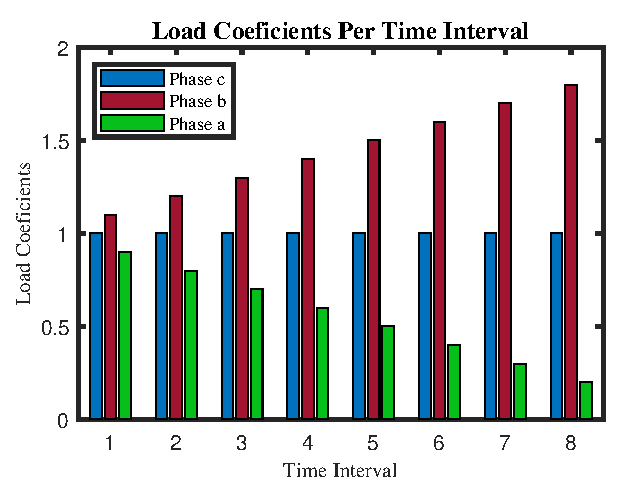
\includegraphics[width=8cm]{pdf/Load Imbalance.pdf}
\vspace*{-0.7cm}
\caption{ Load Imbalance Coeficient per time interval}

\label{Load Imbalance}
\end{figure}
\end{center}
% ================= III. Computational Implementation===============================================
\section{Parameter Tuning} \label{PT}

\subsection {VUF Quadratic Regression}\label{Reg}
In (\ref{VUF_apr_simplified}) the  $\alpha_{i_{mn}}^{\varphi\gamma}$ $\beta_{i_{mn}}^{\varphi\gamma}$
$\delta_{i_{mn}}^{\varphi\gamma}$, can be approximated by a data-driven regression method trained on a VUF results of a set of large data points of voltage angle and magnitude in the operational range. For the purpose of this study the data points are created by sweeping voltage magnitude from $V_{min}=.09$ to $V_{max}=1.1$ with 0.1 increment and angles are swept between $-5^{\circ}$ to $5^{\circ}$ with $1^{\circ}$ increments.  The leveraged data-driven method is the least square multi-variable quadratic regression. Figure \label{VUF_reg} represents the scatter plot of both linear and quadratic regressions. As it can be shown in the figure the although the quadratic regression has a large approximation error due to the high non-linearity of VUF function, it is relatively better that the linear results. Therefore that weighted-sum multiple objective approach is more accurate than hard margin linear VUF implementation. The resultant parameters are embedded to the \textit{OPF VUF} and \textit{Crossphase VUF} methods.
\begin{figure}
\centering
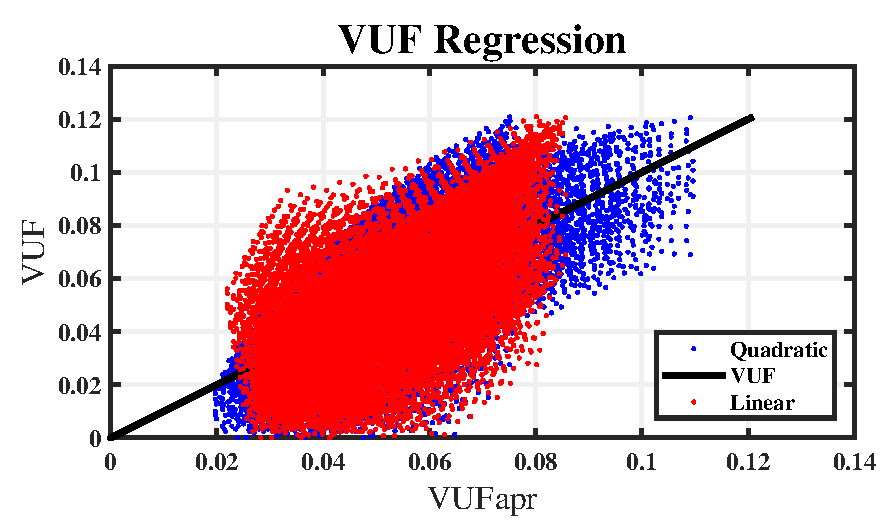
\includegraphics[width=8cm]{pdf/VUF_reg.pdf}
\vspace*{-0.3cm}
\caption{Scatter Plot of Linear and Quadratic Regression of VUF}
\label{VUF_reg}
\end{figure}

\subsection {Pareto Front Trade-Off}\label{Pareto}

In order to enabling a quantified trade-off between cost and sum of VUFs the Pareto method is used.  For having a 2D Pareto Front, it is assumed that all buses have the same weight and $w'=(1-w)$. The Pareto front with 0.1 increments for the \textit{Crossphase VUF} method is illustrated in figure \ref{prt} for the \textit{PVEV afternoon} scenario. it can be seen that for all time intervals there is a significant reduction in sum of VUFs when increasing $w$ from 0 to 0.1. However, further increase of $w$ seems to not have significant decrease in the VUF sum value while it increases the cost drastically. Therefore, the $w=0.1$ is chosen to use in the proposed weighted sum method.

\begin{figure}
\centering
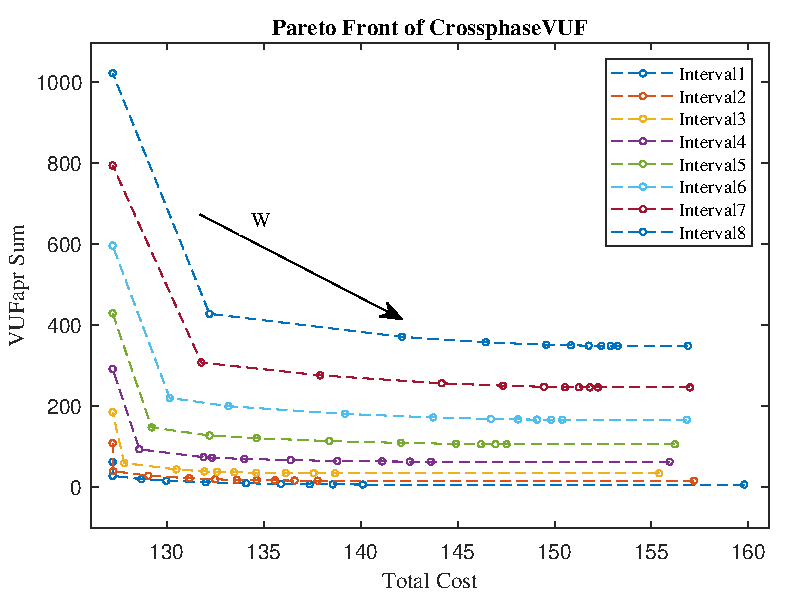
\includegraphics[width=8cm]{pdf/Final.pdf}
\vspace*{-0.3cm}
\caption{Pareto front of \textit{Crossphase VUF} method in \textit{PVEV afternoon} scenario}
\label{prt}
\end{figure}

%====Results and Discussion=================================================================================================

\section {Results and Discussion}

This section compares the effectiveness of the presented sub-methods and scenarios in four aspects; 1) total cost, 2) voltage imbalance, 3)  total loss, and 4) line capacity utilization. For each of the mentioned aspects, first, the \ref{table1} sub-methods are compared in the most complete scenario, \textit{PVEV afternoon}. Then the \ref{scenario_section} scenarios are compared for the state-of-the-art method, \textit{CrossPhase VUF}.

%%%%%%%%%%%%%%%%Table4%%%%%%%%%%%%%%%%%%%%%%%%%%


%%%%%%%%%%%%%%%%%%%%%%%%%%%%%%%%%%%%%%%%%%%%%%%%


%%%%%%%%%%%%%%%%%%%%%%%%%%%%%%%%%%%%%%%%%%%%%%%%%
\subsection{Total cost of the studied systems}

Total cost of the systems for the sub-methods of Table. \ref{table1} is evaluated for the fifth time interval in Table.\ref{Table9}. Assessing the table proves that using a cross-phase enabled sub-method reduces the total cost of the systems in both test systems. As it is visible, utilizing the other sub-methods is not so profitable compared to the \text{cross-phase}. This cost reduction is achieved by exploiting the capacity of PV and EV inverters during operational and non-operational hours in \textit{Crossphase} and \textit{Crossphase VUF} method. Fig. \ref{Cross} shows a comparison between the apparent, active, and reactive power reference of the three-phase EV charger installed on bus number 88 of the IEEE 192 bus system for both \textit{Crossphase} and \textit{OPF} methods during operational and non-operational hours. As it can be shown on the figure, the inverter capacity utilization in operational mode is 5\% more when crossphase is enabled. Moreover, in non-operational hours, crossphase enables the inverter to circulate the active power by consuming power from phase c, and transferring it to phase b to compensate the induced load imbalance shown in figure \ref{Load Imbalance}. Also, as shown in Tables. \ref{Table11}, the total cost of the \textit{Crossphase VUF} is lesser in the scenarios that enables the inverters to contribute in non-operational hours than the scenarios that turn the inverters off during non-operation. This resultant crossphase flexibility, leads to a better optimal solution in terms of cost. It should be mentioned that due to the meshed topology of IEEE 192 bus, enabling crossphase is not guaranteed as in the IEEE 33 bus radial system. This behaviour is related to possible current imbalance propagation to several main lines in meshed grids which is further discussed in \ref{secloss}. Another result that can be obtained from the tables. \ref{Table11} is that although both systems have more PVs in terms of capacity and numbers installed, EVs show a better non-operational crossphase contribution for cost reduction.

Sub-methods that contain a VUF constraint, experience a higher total cost because of the additional term in their objective functions. It can be seen that in both systems intensifying the load imbalance will increase system cost in VUF constrained sub-methods. The cost difference between the VUF-constrained and non constrained sub-methods, is the price that should be paid for compensation of the VUF. 

\begin{center}
\begin{table}
\caption{Total cost of the IEEE systems during “ PV-EV-afternoon” scenario during 5th time interval}
\label{Table9}
\centering

\begin{tabular}{c|c|c|c|c|c}
    \hline\hline
    \multirow{2}[0]{2em}{\textbf{System}} &  \multirow{2}[0]{2em}{\textbf{Fixed}} & \multirow{2}[0]{2em}{\textbf{OPF}} & \multirow{2}[0]{2.5em}{\textbf{OPF-VUF}} & \multirow{2}[0]{5em}{\textbf{Crossphase}} & \multirow{2}[0]{5em}{\textbf{Crossphase-VUF}} \\ & & & & & \\ \hline
    33-Bus & 346.54 & 346.54 & 351.72 & 341.29 & 344.55\\ 
    \hline
    192-Bus & 127.19 & 127.19 & 147.22 & 127.19 & 142.07\\ 
    \hline\hline
    \end{tabular}

\end{table}
\end{center}

%%%%%%%%%%%%%%%%%%%%%%%%%%%%%%%%%%%%%%%%%%%%%%%%%
%%%%%%%%%%%%%%%%%%Table11%%%%%%%%%%%%%%%%%%%%%%%%
%%%
\begin{center}
\begin{table}
\caption{Total cost of the IEEE 33- and 192-Bus systems while implementing Crossphase VUF for different scenarios during 5th time interval}
\label{VUFstandar}
\centering
\setlength{\tabcolsep}{3.5pt}
\begin{tabular}{c|c|c|c|c|c|c}
\hline\hline
 \multirow{2}{3.5em}{Scenarios} &
\multirow{2}{2.8em}{Base (C)} & \multirow{2}{3em}{Base (NC)} & \multirow{2}{3.8em}{EV-Night(C)} & \multirow{2}{3.9em}{EV-Night(NC)} & \multirow{2}{3.9em}{PV-Noon(C)} & \multirow{2}{3.9em}{PV-Noon(NC)}\\
 & & & & & &\\
\hline
\multirow{2}{*}{33-Bus}&
\multirow{2}{*}{361.87} & \multirow{2}{*}{367.81} & \multirow{2}{*}{369.94} & \multirow{2}{*}{373.40} & \multirow{2}{*}{337.35} & \multirow{2}{*}{339.27}\\
 & & & & & & \\ 
\hline
\multirow{2}{*}{192-Bus}&
\multirow{2}{*}{155.19} & \multirow{2}{*}{155.19} & \multirow{2}{*}{171.19}  & \multirow{2}{*}{171.19} & \multirow{2}{*}{126.94} & \multirow{2}{*}{129.92}\\
 & & & & & &\\ 
\hline\hline
    \end{tabular}

\end{table}
\end{center}


%%%%%%%%%%%%%%%%%%%%%%%%%%%%%%%%%%%%%%%%%%%%%%%%%

%%%%%%%%%%%%%%%%%%Table12%%%%%%%%%%%%%%%%%%%%%%%%

%\begin{center}
%\begin{table}
%\caption{Total cost of the IEEE 192-Bus system during different scenarios with Cross-phase-vuf method}
%\label{Table12}
%\centering
%\setlength{\tabcolsep}{2.2pt}
%\begin{tabular}{c|c|c|c|c|c|c|c|c}
%    \hline\hline
%    Hour & 1 & 2 & 3 & 4 & 5 & 6 & 7 & 8\\ \hline
%    Base(C) & 155.19 & 155.19 & 155.19 & 155.19 & 155.19 & 155.19 & 155.19 & 155.19\\
%    \hline
%    \multirow{2}{3.5em}{Base (NC)} & \multirow{2}{*}{155.19} & \multirow{2}{*}{155.19} & \multirow{2}{*}{155.19} & \multirow{2}{*}{155.19} & \multirow{2}{*}{155.19} & \multirow{2}{*}{155.19} & \multirow{2}{*}{155.19} & \multirow{2}{*}{155.19}\\ & & & & & & & &\\
%    \hline
%   \multirow{2}{3.9em}{EV-Night (C)} & \multirow{2}{*}{171.19} & \multirow{2}{*}{171.19} & \multirow{2}{*}{171.19} & \multirow{2}{*}{171.19} & \multirow{2}{*}{171.19} & \multirow{2}{*}{171.19} & \multirow{2}{*}{171.19} & \multirow{2}{*}{171.19}\\ & & & & & & & &\\
%    \hline
%    \multirow{2}{3.9em}{EV-Night (NC)} & \multirow{2}{*}{171.19} & \multirow{2}{*}{171.19} & \multirow{2}{*}{171.19} & \multirow{2}{*}{171.19} & \multirow{2}{*}{171.19} & \multirow{2}{*}{171.19} & \multirow{2}{*}{171.19} & \multirow{2}{*}{171.19}\\ & & & & & & & &\\
%    \hline
%    \multirow{2}{3.9em}{PV-Noon (C)} & \multirow{2}{*}{118.97} & \multirow{2}{*}{118.92} & \multirow{2}{*}{119.31} & \multirow{2}{*}{121.10} & \multirow{2}{*}{126.94} & \multirow{2}{*}{131.45} & \multirow{2}{*}{134.58} & \multirow{2}{*}{136.64}\\ & & & & & & & &\\
%    \hline
%    \multirow{2}{3.9em}{PV-Noon (NC)} & \multirow{2}{*}{121.15} & \multirow{2}{*}{120.70} & \multirow{2}{*}{120.90} & \multirow{2}{*}{123.32} & \multirow{2}{*}{129.92} & \multirow{2}{*}{134.27} & \multirow{2}{*}{138.13} & \multirow{2}{*}{140.28}\\ & & & & & & & &\\
%    \hline\hline
%    \end{tabular}

%\end{table}
%\end{center}

\begin{figure}
\centering
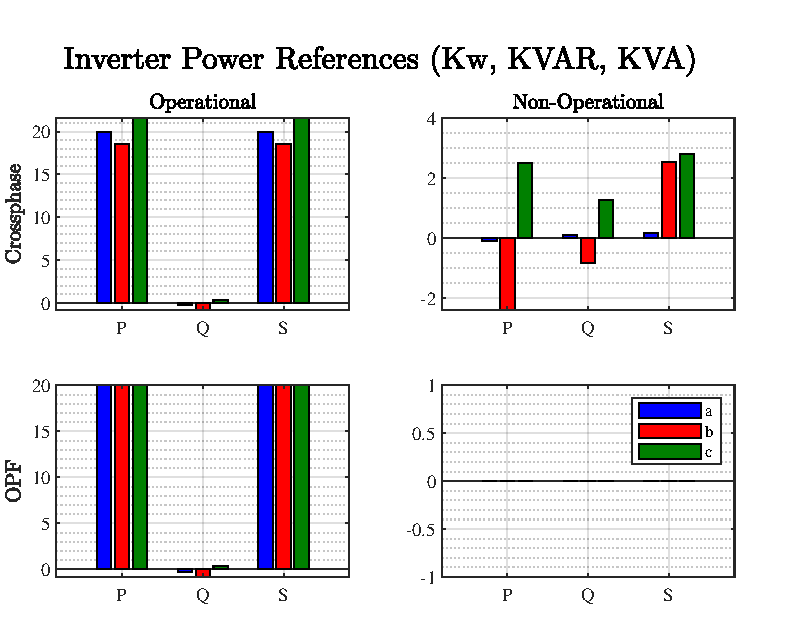
\includegraphics[width=8cm]{pdf/Cross.pdf}
%\vspace*{-0.3cm}
\caption{Comparison Between \textit{Crossphase} and \textit{OPF} Methods in Exploiting the Apparent Power Capacity in a Three-Phase Inverter (EV in bus 89 of 192 bus test system) During Operational and Non-Operational Modes}
\label{Cross}
\end{figure}
%%%%%%%%%%%%%%%%%%%%%%%%%%%%%%%%%%%%%%%%%%%%%%%%%
\subsection{Voltage Imbalance}
Figure \ref{VUF33m} and \ref{VUF192m} compares the results of the VUF for each bus in all time intervals with the mentioed sub-methods of table. \ref{table1}. The results shows the superiority of \textit{crossphase VUF} in reducing the VUF in comparison with others.
Also, the \texit{VUF} \textit{crossphase} show reduction in VUF howeve, the effect of VUF constraint is more than crossphase individully. The \texit{VUF} \textit{OPF} and \textit{Fixed} method that are only different in their lineararity of constraints and solver show a very severe VUF especially in intense time intervals. 

The results for the Scenarios other than \textit{PVEV afternoon} are summarized in table. \ref{VUFstandar}. In this table only the results for the most extreme condition (time interval 8) are shown. According to the table, however the standard could not be maintained in this worst case scenario, the crossphase contribution of EVs and PVs were significantly effective in reducing the nonstandard conditioned buses. Also results reveal that unlike the cost, in terms of VUF reduction, crossphase contribution of PVs in both \textit{Base (C)} and \textit{EV Night (C)} are more effective than crossphase contribution of EVs such that in IEEE 33 bus system they were able to reach a standard solution. The results also reveals that the crossphase capability is more effective in radial 33 bus than heavily meshed 192 bus system.
%%%%%%%%%%%%%%%%%%%%%% fig VUF %%%%%%%%%%%%%%%%%%%%%%%
\begin{figure}
\centering
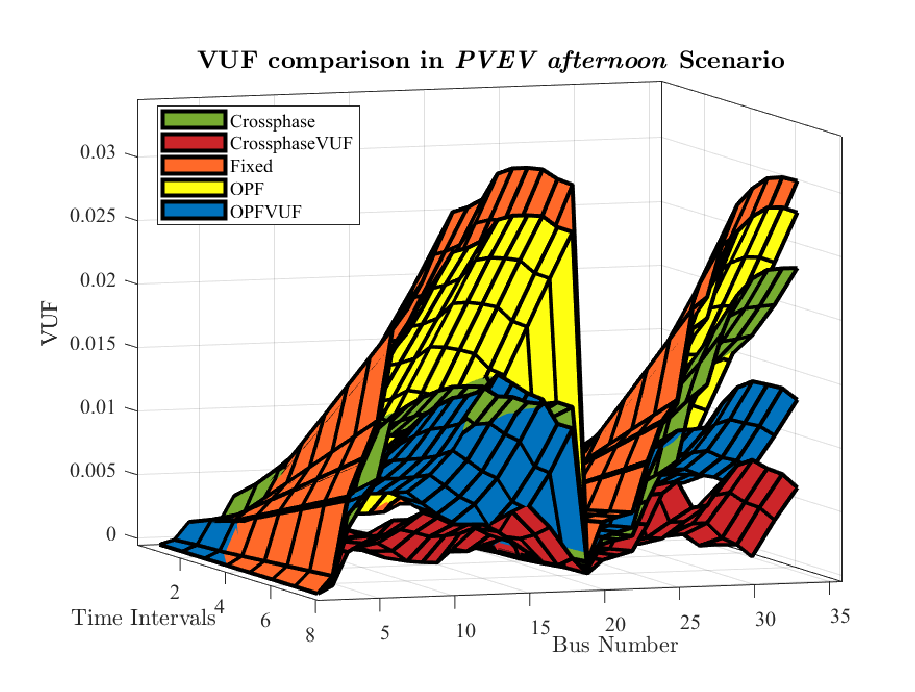
\includegraphics[width=8cm]{pdf/VUF33m.pdf}
\vspace*{-0.3cm}
\caption{VUF Comparison of sub-methods in \textit{PVEV afternoon} scenario in 33 bus system}
\label{VUF33m}
\end{figure}
\begin{figure}
\centering
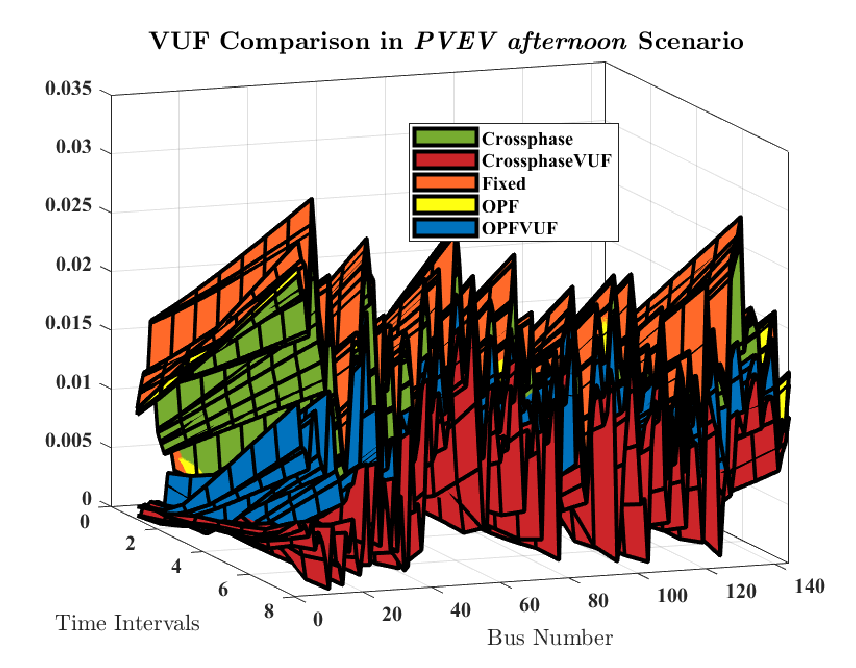
\includegraphics[width=8cm]{pdf/VUF192m.pdf}
\vspace*{-0.3cm}
\caption{VUF Comparison of sub-methods in \textit{PVEV afternoon} scenario in 192 bus system (Slack buses are not shown)}
\label{VUF192m}
\end{figure}


%%%%%%%%%%%%%%%%%%%%%Table15%%%%%%%%%%%%%%%%%%%%%%%%

\begin{center}
\begin{table}
\caption{Percentage of the Buses of IEEE 33 and 192-Bus system violating the IEEE 1159 standard during different scenarios ($\%$)}
\label{VUFstandar}
\centering
\setlength{\tabcolsep}{3.5pt}
\begin{tabular}{c|c|c|c|c|c|c}
\hline\hline
 \multirow{2}{3em}{Test system} &
\multirow{2}{3em}{Base (NC)} & \multirow{2}{3em}{Base (C)} & \multirow{2}{3.8em}{PV-Noon (NC)} & \multirow{2}{3.8em}{PV-Noon (C)} & \multirow{2}{3.9em}{EV-Night (NC)} & \multirow{2}{3.9em}{EV-Night (C)}\\
 & & & & & &\\
\hline
\multirow{2}{*}{33-Bus}&
\multirow{2}{*}{76} & \multirow{2}{*}{0} & \multirow{2}{*}{24} & \multirow{2}{*}{6} & \multirow{2}{*}{69} & \multirow{2}{*}{0}\\
 & & & & & & \\ 
\hline
\multirow{2}{*}{342-Bus}&
\multirow{2}{*}{75} & \multirow{2}{*}{43} & \multirow{2}{*}{46}  & \multirow{2}{*}{41} & \multirow{2}{*}{71} & \multirow{2}{*}{44}\\
 & & & & & &\\ 
\hline\hline
    \end{tabular}

\end{table}
\end{center}

%%%%%%%%%%%%%%%%%%%%%%%%%%%%%%%%%%%%%%%%%%%%%%%%%%%%
\subsection {Total power loss of the test systems}\label{secloss}

Total power loss of the test systems for different sub-methods are pointed out in Tables. \ref{Table5} and \ref{Table6}. Analyzing Table.\ref{Table5} clears that by increasing load imbalance intensity, total power loss of the IEEE 33-Bus system experiences an upward trend. Due to the constant three-phase load power in all intervals, it can be concluded that the the increase in loss is solely a result of increase in the line imbalance. Before discussing the relation between line imbalance and crossphase, it needs to be mentioned that the crossphase opeartion for the cost and VUF minimization can have two forms: 1) allocating power of the inverter in order to meet the unbalanced load demand. 2) transferring flowing power probably generated from a collection of single-phase PVs in one phase to another. The first form will locally compensate the line imbalance of the lower side and can have a balancing effect on the upper main line in radial systems. The latter however will exploit the line capacity to transfer a generated single phase power to the upper side loads or loads in the other phases and therefore my not guarantee a balanced upper main line balance. By taking the above mentioned into consideration, it can be seen that on table. \ref{Table5} when the loads are nearly balanced (intervals 1-3) \textit{crossphase VUF} compromises the the line imbalance and the loss to reach a better VUF and cost, however in the highly unbalanced situations, the \textit{crossphase VUF} minimizes the VUF and cost without any need to compromise the loss. Therefore in these cases both current and voltage imbalance are minimized alongside with the cost. Analysing the results of table. \ref{Table6} with the same manner reveals that in the presented heavily meshed grid, the loss in \textit{crossphase VUF} is more than \textit{crossphase} in all time intervals which means that the line imbalance most be compromised to reach a better VUF. This behaviour is like the behaviour of the radial grid between (1-3) intervals. Therefore it can be concluded that the voltage and current imbalance are not always inlined.

The scenario based results are presented in tables \ref{Table7} and \ref{Table8}. According to 33 Bus system results, non-operational contribution of EVs and PVs both worked in favor of the system loss reduction in all intervals which illustrates the superiority of cross phasing in radial topology in terms of loss. In analysing different conclusions can be made. First, comparing the results of \textit{Base (NC)} and \textit{(C)} for interval 1 where there is no single-phase generation reveals that attempt to reduce VUF and cost will propagate line imbalance due to meshed topology. This result shows that the claim made for the first form of cross-phasing is not valid in meshed networks. Second, in comparing results of \textit{EV Night (NC)} and \textit{(C)}, where the cross phasing is dine by PVs and a lot of single-phase generation exists, loss reduction will not occur before interval 7 which supports the claim made in the previous paragraph about the second form of cross-phasing. On the other hand, \textit{ PV noon (NC)} and \textit{(C)} shows that only EV cross-phasing in full presence of PVs was able to reduce the loss in all time intervals successfully. 

%%%%%%%%%%%%%%%%%%%%%Table5%%%%%%%%%%%%%%%%%%%%%%
\begin{center}
\begin{table}
\caption{Total power loss in IEEE 33-Bus system with different dispatching methods (kW)}
\label{Table5}
\centering

\begin{tabular}{c|c|c|c|c|c}
    \hline\hline
    \multirow{2}[0]{*}{\textbf{Hour}} &  \multirow{2}[0]{*}{\textbf{Fixed}} & \multirow{2}[0]{*}{\textbf{OPF}} & \multirow{2}[0]{*}{\textbf{OPF-VUF}} & \multirow{2}[0]{*}{\textbf{Crossphase}} & \multirow{2}[0]{5em}{\textbf{Crossphase-VUF}} \\ & & & & & \\ \hline
    1 & 4.88 & 4.87 & 4.68 & 4.86 & 5.01\\ 
    \hline
    2 & 4.98 & 4.97 & 4.81 & 4.92 & 5.05\\ 
    \hline
    3 & 5.15 & 5.14 & 5.13 & 5.06 & 5.16\\ 
    \hline
    4 & 5.39 & 5.37 & 5.35 & 5.26 & 5.32\\ 
    \hline
    5 & 5.70 & 5.69 & 5.60 & 5.54 & 5.56\\ 
    \hline
    6 & 6.08 & 6.07 & 5.91 & 5.88 & 5.86\\ 
    \hline
    7 & 6.53 & 6.52 & 6.29 & 6.29 & 6.22\\ 
    \hline
    8 & 7.06 & 7.04 & 6.75 & 6.78 & 6.66\\ 
    \hline\hline
    \end{tabular}

\end{table}
\end{center}

%%%%%%%%%%%%%%%%%%%%%%%%%%%%%%%%%%%%%%%%%%%%%%%%%

%%%%%%%%%%%%%%%%%%%%%%Table6%%%%%%%%%%%%%%%%%%%%%

\begin{center}
\begin{table}
\caption{Total power loss in IEEE 192-Bus system with different dispatching methods (kW)}
\label{Table6}
\centering

\begin{tabular}{c|c|c|c|c|c}
    \hline\hline
    \multirow{2}[0]{*}{\textbf{Hour}} &  \multirow{2}[0]{*}{\textbf{Fixed}} & \multirow{2}[0]{*}{\textbf{OPF}} & \multirow{2}[0]{*}{\textbf{OPF-VUF}} & \multirow{2}[0]{*}{\textbf{Crossphase}} & \multirow{2}[0]{5em}{\textbf{Crossphase-VUF}} \\ & & & & & \\ \hline
    1 & 14.15 & 14.40 & 15.51 & 14.42 & 14.80\\ 
    \hline
    2 & 14.47 & 14.72 & 16.11 & 14.72 & 14.82\\ 
    \hline
    3 & 15.00 & 15.25 & 16.62 & 15.24 & 15.14\\ 
    \hline
    4 & 15.74 & 16.00 & 17.16 & 15.95 & 15.99\\ 
    \hline
    5 & 16.70 & 16.94 & 17.85 & 16.86 & 17.29\\ 
    \hline
    6 & 17.87 & 18.07 & 18.72 & 17.92 & 18.53\\ 
    \hline
    7 & 19.25 & 19.43 & 19.81 & 19.29 & 19.79\\ 
    \hline
    8 & 20.85 & 21.00 & 21.09 & 20.81 & 20.97\\ 
    \hline\hline
    \end{tabular}

\end{table}
\end{center}

%%%%%%%%%%%%%%%%%%%%%%%%%%%%%%%%%%%%%%%%%%%%%%%%%

%%%%%%%%%%%%%%%%%%%%Table7%%%%%%%%%%%%%%%%%%%%%%%

\begin{center}
\begin{table}
\caption{Total power loss of the 33-Bus system with crossphase-vuf method during different scenarios (kW)}
\label{Table7}
\centering
\setlength{\tabcolsep}{5.5pt}
\begin{tabular}{c|c|c|c|c|c|c|c|c}
    \hline\hline
    Hour & 1 & 2 & 3 & 4 & 5 & 6 & 7 & 8\\ \hline
    Base(C) & 5.22 & 5.20 & 5.09 & 5.37 & 5.69 & 5.83 & 5.98 & 6.11\\
    \hline
    \multirow{2}{3.5em}{Base (NC)} & \multirow{2}{*}{5.31} & \multirow{2}{*}{5.41} & \multirow{2}{*}{5.59} & \multirow{2}{*}{5.83} & \multirow{2}{*}{6.15} & \multirow{2}{*}{6.53} & \multirow{2}{*}{6.99} & \multirow{2}{*}{7.51}\\ & & & & & & & &\\
    \hline
   \multirow{2}{3.9em}{EV-Night (C)} & \multirow{2}{*}{5.87} & \multirow{2}{*}{5.74} & \multirow{2}{*}{5.66} & \multirow{2}{*}{5.78} & \multirow{2}{*}{6.31} & \multirow{2}{*}{6.66} & \multirow{2}{*}{6.49} & \multirow{2}{*}{6.76}\\ & & & & & & & &\\
    \hline
    \multirow{2}{3.9em}{EV-Night (NC)} & \multirow{2}{*}{6.27} & \multirow{2}{*}{6.06} & \multirow{2}{*}{6.03} & \multirow{2}{*}{6.17} & \multirow{2}{*}{6.38} & \multirow{2}{*}{6.66} & \multirow{2}{*}{7.01} & \multirow{2}{*}{7.40}\\ & & & & & & & &\\
    \hline
    \multirow{2}{3.9em}{PV-Noon (C)} & \multirow{2}{*}{2.43} & \multirow{2}{*}{2.68} & \multirow{2}{*}{3.12} & \multirow{2}{*}{3.35} & \multirow{2}{*}{3.32} & \multirow{2}{*}{3.07} & \multirow{2}{*}{3.89} & \multirow{2}{*}{4.48}\\ & & & & & & & &\\
    \hline
    \multirow{2}{3.9em}{PV-Noon (NC)}  & \multirow{2}{*}{2.80} & \multirow{2}{*}{2.79} & \multirow{2}{*}{2.85} & \multirow{2}{*}{2.96} & \multirow{2}{*}{3.23} & \multirow{2}{*}{3.67} & \multirow{2}{*}{4.46} & \multirow{2}{*}{5.06}\\ & & & & & & & &\\
    \hline\hline
    \end{tabular}

\end{table}
\end{center}

%%%%%%%%%%%%%%%%%%%%%%%%%%%%%%%%%%%%%%%%%%%%%%%%%
%%%%%%%%%%%%%%%%%%%%Table8%%%%%%%%%%%%%%%%%%%%%%%

\begin{center}
\begin{table}
\caption{Total power loss of the 192-Bus system with crossphase-vuf method in different scenarios (kW)}
\label{Table8}
\centering
\setlength{\tabcolsep}{4pt}
\begin{tabular}{c|c|c|c|c|c|c|c|c}
    \hline\hline
    Hour & 1 & 2 & 3 & 4 & 5 & 6 & 7 & 8\\ \hline
    Base(C) & 16.72 & 16.85 & 17.17 & 17.79 & 18.53 & 19.35 & 20.31 & 21.38\\
    \hline
    \multirow{2}{3.5em}{Base (NC)} & \multirow{2}{*}{16.48} & \multirow{2}{*}{16.79} & \multirow{2}{*}{17.32} & \multirow{2}{*}{18.06} & \multirow{2}{*}{19.00} & \multirow{2}{*}{20.16} & \multirow{2}{*}{21.53} & \multirow{2}{*}{23.11}\\ & & & & & & & &\\
    \hline
   \multirow{2}{3.9em}{EV-Night (C)} & \multirow{2}{*}{19.85} & \multirow{2}{*}{20.02} & \multirow{2}{*}{20.38} & \multirow{2}{*}{21.01} & \multirow{2}{*}{21.77} & \multirow{2}{*}{22.64} & \multirow{2}{*}{23.57} & \multirow{2}{*}{24.69}\\ & & & & & & & &\\
    \hline
    \multirow{2}{3.9em}{EV-Night (NC)} & \multirow{2}{*}{19.60} & \multirow{2}{*}{19.77} & \multirow{2}{*}{20.17} & \multirow{2}{*}{20.79} & \multirow{2}{*}{21.59} & \multirow{2}{*}{22.58} & \multirow{2}{*}{23.77} & \multirow{2}{*}{25.18}\\ & & & & & & & &\\
    \hline
    \multirow{2}{3.9em}{PV-Noon (C)} & \multirow{2}{*}{12.52} & \multirow{2}{*}{12.70} & \multirow{2}{*}{12.98} & \multirow{2}{*}{13.64} & \multirow{2}{*}{14.93} & \multirow{2}{*}{16.12} & \multirow{2}{*}{17.30} & \multirow{2}{*}{18.46}\\ & & & & & & & &\\
    \hline
    \multirow{2}{3.9em}{PV-Noon (NC)} & \multirow{2}{*}{12.68} & \multirow{2}{*}{12.87} & \multirow{2}{*}{13.32} & \multirow{2}{*}{14.24} & \multirow{2}{*}{15.68} & \multirow{2}{*}{16.97} & \multirow{2}{*}{18.40} & \multirow{2}{*}{19.77}\\ & & & & & & & &\\
    \hline\hline
    \end{tabular}

\end{table}
\end{center}


%\subsection{Line Capacity Utilization}
%Capacity equation%
%Line capacity Utilization means that how much of

%\begin{equation}
%    \label{Capacity_Relief}
%    \displaystyle\sum _{(i,j)=1-l} (S_{ij} - APM_{ij})
%\end{equation}
%Comparing the derived amounts in Table. \ref{Table17} declares that utilizing the Crossphase-VUF method maximizes the total empty capacity of the test systems. Moreover, the positive impact of power displacing through phases is visible in different scenarios reported in Table. \ref{Table19}.

%%%%%%%%%%%%%%%%%%%%%%Table17%%%%%%%%%%%%%%%%%%%%%%%

%\begin{center}
%\begin{table}
%\caption{The amount of MCR while using different methods in IEEE 33 and 342-Bus system (kVA)}
%\label{Table17}
%\centering
%\setlength{\tabcolsep}{2.7pt}
%\begin{tabular}{c|c|c|c|c|c}
%\hline\hline
%\multirow{2}{*}{\textbf{Test system}} &
%\multirow{2}{*}{\textbf{Fixed}} & \multirow{2}{*}{\textbf{OPF}} & \multirow{2}{*}{\textbf{OPF-VUF}} & \multirow{2}{*}{\textbf{Crossphase}} & \multirow{2}{*}{\textbf{Crossphase-VUF}}\\
% & & & & &\\
%\hline
%\multirow{2}{*}{33-Bus} &
%\multirow{2}{*}{186.13} & \multirow{2}{*}{186.26} & \multirow{2}{*}{188.59} & \multirow{2}{*}{187.88} & \multirow{2}{*}{189.33}\\
% & & & & &\\
%\hline
%\multirow{2}{*}{342-Bus} &
%\multirow{2}{*}{19.20} & \multirow{2}{*}{19.19} & \multirow{2}{*}{19.52} & \multirow{2}{*}{19.24} & \multirow{2}{*}{19.76}\\
% & & & & &\\
%\hline\hline
%    \end{tabular}

%\end{table}
%\end{center}

%%%%%%%%%%%%%%%%%%%%%%%%%%%%%%%%%%%%%%%%%%%%%%%%%%%%

%%%%%%%%%%%%%%%%%%%%%Table19%%%%%%%%%%%%%%%%%%%%%%%%

%\begin{center}
%\begin{table}
%\caption{The MCR amount of the IEEE 33 and %342-Bus system during different scenarios %(kVA)}
%\label{Table19}
%\centering
%\setlength{\tabcolsep}{3.5pt}
%\begin{tabular}{c|c|c|c|c|c|c}
%\hline\hline
%\multirow{2}{2.7em}{Test system}&
%\multirow{2}{2em}{Base (NC)} & \multirow{2}{2em}{Base (C)} & \multirow{2}{3.9em}{PV-Noon (NC)} & %\multirow{2}{3.9em}{PV-Noon (C)} & %\multirow{2}{3.9em}{EV-Night (NC)} & %\multirow{2}{3.9em}{EV-Night (C)}\\
% & & & & & &\\
%\hline
%\multirow{2}{*}{33-Bus} &
%\multirow{2}{*}{184.20} & \multirow{2}{*}{189.72} & \multirow{2}{*}{188.38} & \multirow{2}{*}{189.41} & %\multirow{2}{*}{185.16} & %\multirow{2}{*}{188.22}\\
% & & & & & &\\ 
%\hline
%\multirow{2}{*}{342-Bus} &
%\multirow{2}{*}{18.42} & %\multirow{2}{*}{19.33} & %\multirow{2}{*}{19.38} & %\multirow{2}{*}{19.95} & %\multirow{2}{*}{18.34} & %\multirow{2}{*}{18.62}\\
% & & & & & &\\ 
%\hline\hline
%    \end{tabular}

%\end{table}
%\end{center}

%%%%%%%%%%%%%%%%%%%%%%%%%%%%%%%%%%%%%%%%%%%%%%%%%%%%



%%%%%%%%%%%%%%%%%%%%%%%%%%%%%%%%%%%%%%%%%%%%%%%%%%%
%Magadire hamaye jadvalha check shavand.
%%%%%%%%%%%%%%%%%%%%%%%%%%%%%%%%%%%%%%%%%%%%%%%%%%%%


%Conclusion%==============================================================================================================

\section{Conclusion}

In this paper an exact three-phase optimal power flow that includes both voltage angle and magnitude (AC load load flow) that also works in meshed networks is introduced to be able to optimally manage the per phase active and reactive power references of single and three phase PVs and EVs. The consideration of voltage angle and magnitude enabled the optimal power flow to include the VUF as an operational constraint/objective. In addition, in order to guarantee a good computational performance, all the optimal power flow and constraints are linearized and VUF constrained is approximated with a second degree multi-variable polynomial by regression over an inclusive data set in the operational range of voltage magnitudes and angles. This considerations led to a quadratic formulation of three-phase optimal power flow that can be solved by fast convex solvers. In addition, the cross-phase capability of three-phase EVs and PVs are implemented into formulations to fully exploit the inverter capacity to minimize cost and fix the VUF. This crossphase capability can also be profitable in non-operational modes of PVs and EVs.  Later on, in order to better integrate VUF and cost minimization, a Pareto front trade-off has been made. In order to show the the effect of both including VUF constraint and cross-phase capability in operational and non-operational modes, multiple sub-methods and scenario are tested in terms of total cost, total loss, and VUF reduction in IEEE 33 bus radial and IEEE 192 heavily meshed systems.

The method comparison results revealed that using a cross-phase enabled sub-methods reduces the total cost of the systems in both test systems and the Sub-methods. This reduction is the cost that an inverter owner saves for DSO by enabling the cross-phase capability. Also sub-methods containing a VUF constraint, experience a higher total cost because of the additional term in their objective functions while showing a superiority reducing the VUF. Therefore, the cost difference between the VUF-constrained and non constrained sub-methods, is the price that should be paid for compensation of the VUF. In terms of loss, by increasing load imbalance intensity, total power loss of the systems which is closely related to line imbalance due to normalized implementation of load imbalance experienced an upward trend with increase in load imbalance. When the loads were nearly balanced \textit{crossphase VUF} compromised the the line imbalance to obtain a better VUF and cost, however in the
highly unbalanced situations, the \textit{crossphase VUF} minimized
the VUF and cost without any need to compromise the line imbalance. In terms of scenario comparison, results for multiple scenarios showed that enabling non-operational cross-phase leads to a better optimal solution in terms of cost and is significantly effective in reducing the VUF. 

Finally, as a device based comparison, EVs show a better non-operational cross-phase contribution for cost reduction. however, in terms of VUF reduction, it is vise versa.

%%%%%%%%%%%%%%%%%%%%%%%%%%%%%%%%%%%%%%%%%%%%%%%%%%%%%%%%%%%%%

\bibliography{bibliography}
\bibliographystyle{IEEEtran}

\end{document}